%!TEX root = ../thesis.tex

\chapter{Introduction}\label{cha:introduction}

\section{Towards the characterization of exoplanets}

The field of exoplanetary science is rapidly accelerating.
Large scientific and instrumental investments have been undertaken, with the ultimate goal of detecting and characterizing an Earth-like planet that has the potential for life (as we know it).
Since the very first exoplanet detection around a Sun-like star~\citep{mayor_jupitermass_1995} the number of confirmed exoplanets has grown to over 3872 with another 2898 candidates awaiting confirmation as of January~2019\footnote{\href{https://exoplanets.nasa.gov/}{\url{https://exoplanets.nasa.gov}}.}.
A planet transitions from a ``candidate'' to ``confirmed'' when the probability of false positives is very low, usually achieved using advanced analysis techniques and/or complementary measurements from other detection methods.
However, simply detecting the presence of exoplanets is not nearly enough to satisfy our quest for knowledge.
There is an exorbitant amount of insight to be gained through the full characterization of these known exoplanets, such as: density, composition, internal structure, atmosphere properties, and surface temperature.

When a new extra-solar planet is suspected, follow-up observation and analysis is required to confirm its existence, and its properties.
In particular for the highly sought after Earth-twin, a full characterization is required to determine their habitability.
Notability, here have been several small planets, which have had early claims of Earth-twin status, later determined to be false (or fall below a 99\% probability level) after follow up investigation~\citep[e.g.][]{mullally_kepler_2018,burke_reevaluating_2019}, and the presence of some exoplanets have been heavily debated in literature such as {Gliese~581g}~\citep{vogt_lickcarnegie_2010, gregory_bayesian_2011,robertson_stellar_2014}.
Detecting and analysing exoplanet atmospheres aid in the characterization of exoplanets by allowing their temperature, atmospheric structure, the presence of any scattering aerosols, and the chemical composition to be determined~\citep[e.g.][and references therein]{kreidberg_exoplanet_2018}.
%\todo{references here would be nice}.%exoplanet handbook is a cop-out due to time
All providing clues towards a full exoplanet characterization.

There are several new developments for detecting and characterisation of new exoplanetary systems. For instance, the new space-based transit missions such as {TESS}, {PLATO} and {CHEOPS}.
One of the more promising ground-based approaches is high-resolution near-infrared (\nir{}) spectroscopy.
Several new \nir{} spectrographs are in development~\citep[e.g.][]{wright_third_2017} primarily to detect and characterize exoplanets around cooler {M-dwarf} stars. The \nir{} wavelengths are closer to the peak emissions of cooler stars and exoplanets, while the smaller mass and radius of {M-dwarfs} allow exoplanets to induce larger relative signals that are relatively easier to detect.

In this chapter the common exoplanet and atmospheric detection methods will be introduced, followed by some exoplanet property distributions and the motivation for the work performed in this thesis.

%!TEX root = ../../thesis.tex

\section{Exoplanet detection methods}
\label{sec:detection_methods}
There are several detection methods used to build up the picture of the current understanding of exoplanet candidates.
The different detection methods are often complementary, in that they are sensitive to different parameter spaces and are able to contribute different exoplanet properties, or detect different classes of exoplanet.
The simplest example is that planetary mass and radius are obtained from the radial velocity and transit methods separately.
Also the transit and radial velocity methods are both sensitive to large planets close to the star however, the direct imaging technique cannot see planets too close to the star, as the planets image is contaminated by the stellar image and speckles.

The exoplanet detection rates for different methods since 1995 are shown in \cref{fig:detection_year_method}.
The detection rates among different methods are not uniform, with the transit method having the majority of detections due to the use of the Kepler space telescope~\citep{borucki_finding_2008}.
The radial velocity method has a fairly consistent detection rate, while direct imaging and other methods have only made a small contribution to the total number of detections so far.
Details about the various main detection methods are provided in the following sections.

\begin{figure}
    \centering
    \includegraphics[width=0.7\linewidth]{./figures/introduction/exoplanetEU_year_method.pdf}
    \caption[Number of exoplanet detections per year separated by method.]{Number of exoplanet detections per year separated by method (data from \href{http://ww.exoplanet.eu}{exoplanet.eu} October 2018).}
    \label{fig:detection_year_method}
\end{figure}
\todo{Adjust figure so that can be seen in black and white, textures on bars?}
\subsection{Radial Velocimetry}
\label{subsec:radial_velocimetry}
This technique measures the radial velocity\footnote{Velocity projected along line of sight.} (RV) of the star by analysing the relative Doppler shift of its spectral lines due to the gravitational interaction with a companion.
As the star and companion orbit around their common centre of mass (barycentre) the spectrum of the star periodically oscillates, with the orbital period of the planet, due to the change in relative motion to the observer as depicted in \cref{fig:rvdiagram-mayor} (left).

\begin{figure}
    \centering
    \includegraphics[height=5cm]{./figures/introduction/RV_Diagram}
    \includegraphics[height=5cm]{./figures/introduction/PhaseFolded_51Pegb_Mayor_et_al_1995}
    \caption[The {RV} method.]{Left: Diagram of {RV} method.
    Right: {RV} variation for the detection of {51 Pegasi}.
    Credit:~\citet{mayor_jupitermass_1995}}.
    \label{fig:rvdiagram-mayor}
\end{figure}

The radial velocity variation, directed along the line of sight, is given by:
\begin{equation}
\label{eqn:rv_equation_intro}
{RV} = \gamma + K [\cos{(\nu(t, P, T_0, e) + \omega)} + e\cos{(\omega)}]
\end{equation}
where \(\gamma\) is constant barycentre velocity of the system relative to the Sun\footnote{Earth's barycentre motion is well known and removed.}, \(K\) is the velocity semi-amplitude, \(e\) the eccentricity, and \(\omega\) is the argument of periastron.
The true anomaly \(\nu\), is a function of time \(t\), orbital period \(P\), and the time of periastron passage \(T_0\), and eccentricity.

The velocity amplitude $K$ of a star of mass $\Mstar$ due to a companion with mass $\Mp$ with orbital period $P$, eccentricity $e$, and inclination\footnote{Relative to a plane that is tangential to the celestial sphere, $i=90$ is edge on.} $i$ is~\citep[e.g.][]{cumming_lick_1999}:
\begin{equation}
    K = {\left(\frac{2\pi G}{P}\right)}^{1/3} \frac{\Mp{} \sin{i}}{{(\Mp{} + \Mstar)}^{2/3}} \frac{1}{\sqrt{1-{e}^{2}}}, \label{eqn:k_amplitude}
\end{equation}
where G is the gravitational constant.

The key exoplanet property determined by the amplitude {RV} technique is the companion mass, relative to the orbital inclination \Mpsini.
As the companion mass is in the numerator of \cref{eqn:k_amplitude} the {RV} technique is more sensitive to larger mass planets.
Also since $K \propto P^{-1/3}$ the amplitude is greater for short period close in orbits\footnote{From Kepler's Law ${P}^{2}\propto {a}^{3}$}.

\begin{figure}
    \centering
    \includegraphics[width=0.7\linewidth]{figures/introduction/exoplanetEU_year_mass.pdf}
    \caption[Exoplanet discovery year verses exoplanet mass.]{Exoplanet discovery year verses exoplanet mass showing a trend towards detecting lower mass planets.
    Exoplanets without a measured mass are not shown.
    The colours indicate the initial detection method.}
    \label{fig:exoplaneteuyearmass}
\end{figure}

The {RV} method kick-started the exoplanet discipline by detecting the first exoplanet around a solar-type star {51 Pegasi}~\citep{mayor_jupitermass_1995}.
The {RV} curve for {51 Pegasi} is shown on the right side of \cref{fig:rvdiagram-mayor}.
The first discoveries were surprising as Jupiter mass planets in short period orbits\footnote{\Mpsini=0.47\,\Mjup{} orbiting at 0.05\AU{} for {51 Pegasi}} were unlike anything in our Solar System and not predicted by standard plant formation theories.
Several exoplanet discoveries followed in quick succession~\citep[e.g.][]{butler_planet_1996, marcy_planetary_1996} with many confirming the existence of the type of planets now referred to as ``hot-Jupiters''~\citep{butler_three_1997, charbonneau_detection_2000}.

The radial velocity amplitudes of the first exoplanets detected were around 60\mps{} while
the radial velocity signal of the Earth in a one year orbit around a solar-type star however is 8.9\cmps{}~\citep[e.g.][]{figueira_radial_2010}.
Dedicated spectrographs, such as HARPS~\citep{mayor_setting_2003} along with improved reduction techniques~\citep{lovis_new_2007} pushed this mass detection limit down to the \mps{} level.
ESPRESSO~\citep{pepe_espresso_2014, megevand_espresso_2014} is the next generation high precision optical spectrograph aiming to push the detection limits to 10\cmps, to detect an Earth twin.
The gradual decrease in measured mass of exoplanets over time is shown in \cref{fig:exoplaneteuyearmass}.
The different symbols indicate the detection method, not necessarily the method used to measure the exoplanet mass.

Most {RV} detection has been performed using optical spectrographs.
However, as the amplitude of {RV} signal is inversely proportional to the mass of the star (RV $\propto \Mstar^{-2/3}$), there are dedicated surveys focusing on smaller mass M-dwarf stars~\citep[e.g.][]{reiners_carmenes_2018}.
M-dwarfs are inherently cooler and thus emit a majority of their stellar output in the near-infrared.
New dedicated high-resolution \nir{} spectrographs have and are being designed and implemented to meet this demand e.g.\ {CARMENES}, {NIRPS}, {SPIRou}, {CRIRES+}.


\subsection{Transit methods}
\label{subsec:transit}
The transit method detects the presence of an exoplanet by observing the periodic dimming of the star due to the passage of the exoplanet between the star and observer, partially blocking the star.
Geometry requires the orbit of the exoplanet to be aligned edge-on to the line of sight (low inclinations) for a transit to occur.
The geometric probability, $P$, that a exoplanet transits is estimated by
\begin{equation}
P \approx \frac{\Rstar}{a (1-{e}^{2})},
\end{equation}
where \(e\) is the eccentricity of the orbit, $\Rstar$ is the star radii and \(a\) is the semi-major axis of the orbit (star-planet distance)~\citep[e.g.][]{barnes_effects_2007}.
The probability of transit increases with the size of the star but decreases with distance to the star.

The drop in stellar brightness during the transit allows the measurement of the planet/star radius ratio:
\begin{equation}
    \frac{\Delta L}{L}\sim{\left(\frac{\Rp}{\Rstar}\right)}^{2}
\end{equation}
where \(L\) is the luminosity of the star, \(\Delta L\) is the maximum luminosity variation (transit depth), and \(\Rstar\) and \(\Rp\) are the radius of the star and planet respectively.

The transit method complements {RV} measurements as the inclination, $i$, of the orbit can be determined from the transit.
This removes the {$\sin{i}$} ambiguity found in the \Mpsini{} of {RV} detections so the true mass, $\Mp$, of the exoplanet can be revealed.
The true mass along with the planet's radius provides a value for the exoplanets average density\footnote{$\rho \equiv \frac{\textrm{Mass}}{\textrm{Volume}} = \frac{3}{4\pi}\frac{\Mp}{\Rp^{3}}$}, hinting at the possible composition.

There are several other astrophysical phenomena which can mimic transiting exoplanet signals, created by configurations of two or more stars which may not involve an exoplanet.
For example a transiting low-mass or white-dwarf star, grazing binary stars, or a transit in a multi-star system~\citep[see e.g.][]{cameron_extrasolar_2012, santerne_contribution_2013}.
Follow-up {RV} observations~\citep[e.g.][]{santerne_radial_2011} are usually required to confirm the planets existence.
Statistical validation techniques are also possible, such as the PASTIS software~\citep{diaz_pastis_2014}, when follow-up can not be performed.
These techniques assess the likelihood of the planet being a true planet against the different false positive scenarios, validating or confirming the planet if the likelihood is high enough.

The transit method has the highest false positive rate among the detection methods presented here.
With {RV} follow-up,~\citet{santerne_sophie_2012} found a false positive rate as high as 35\% for short period giant planets, while~\citet{santerne_sophie_2016} found a 54.6\% false positive rate of 129 giant planets with periods less than 400 days.
These sub-sample false positive rates are however higher than the global false positive rate of 9.4\%~\citep{fressin_false_2013}/11.3\%~\citep{santerne_contribution_2013} found for Kepler.
Some of the currently known exoplanet systems with the smallest radii and lightest mass have been detected through transit and later confirmed with high-precision {RV} follow-up~\citep[e.g.][]{queloz_corot7_2009, pepe_earthsized_2013, lopez-morales_kepler21b_2016, ment_second_2018}.

The identification of unresolved multiple stars, such as a binary or an unrelated background star, can be achieved through high-resolution spectroscopy in which the spectral lines of individual stars can be separated~\citep{kolbl_detection_2015}.
This is important to measure the correct radii of exoplanets as the extra light contribution from an unresolved secondary star will reduce the transit depth, mimicking a smaller transiting planet.

The transit of a single planet can not directly determine the planetary mass.
However, in multiple planet systems, the masses and sometimes the presence of other planets in the system can be determined from perturbations in the transit time and duration~\citep[e.g.][]{holman_use_2005, holman_kepler9_2010}.
A large number of systems have been detected that show transit timing variations (TTV) and transit duration variations (TDV)~\citep[e.g.][]{holczer_transit_2016} due to the gravitational interaction between planets.
The statistical validity of multi-transiting planets is more straightforward than single planets as the probability of having multiple false positives, being the product of the individual probabilities, is lower than having multiple planets in the system~\citep{lissauer_almost_2012}, making multiple planet systems easier to validate.

The presence of star spots on the surface of a star can be observed during transit.
A star spot is a dark region on the stellar surface due to magnetic fields, which decreases the luminosity slightly.
Examples of spots can be seen in the middle of the Sun from an image of the 2012 transit of Venus in \cref{fig:transit_venus_transit_alignment} (left).
It shows several dark sunspots alongside Venus, although Venus did not cross them.
Unlike for other stars, sunspots are spatially resolved.
If an exoplanet passes in front of a spot, the luminosity decrease from the spot is temporarily hidden and a small bump occurs in the transit shape.
The presence of spots in successive transits (see \cref{fig:transit_venus_transit_alignment} (right)) can indicate the alignment of the stellar rotation to the planet orbital plane~\citep{sanchis-ojeda_starspots_2013}.
In this simulation an orbit aligned with the stellar rotation and the transit crosses the spot in four successive orbits.
In a misaligned case a spot would only be observed in one transit.

\begin{figure}
    \centering
    \includegraphics[height=5cm]{./figures/introduction/SDO_2012_Venus_Transit.jpg}
    \includegraphics[height=5cm]{figures/introduction/sanchisojedafig1-crop.pdf}
    \caption[Transit of Venus and successive transit corssings.]{Left: Image from the 2012 transit of Venus obtained from the Solar Dynamics Observatory satellite.
    Venus is the dark circle in the top left of the Sun.
    Limb darkening is observed as the change in colour/brightness from white to red near the edge.
    Several sunspots are also observed on the surface of the Sun.
    Credit: {NASA}/{SDO}, {HMIR}.
    Right: Simulation of 4 successive transits crossing a star spot with the orbit aligned with the stellar rotation.
    The stellar rotation is 1/10 the orbital period.
    Adapted from~\citet[][Figure~1]{sanchis-ojeda_starspots_2013}.}
    \label{fig:transit_venus_transit_alignment}
\end{figure}


The vast majority of transit detections have come from Kepler~\citep{borucki_characteristics_2011}, which focused on a small patch of sky (0.25\%) for four years continuously.
Kepler's impressive sensitivity compared to previous surveys, allowed it to detect planets down to around 2\Rearth.
However, {CoRoT}~\citep{barge_transiting_2008} and ground-based surveys, such as WASP~\citep{pollacco_wasp_2006}, OGLE~\citep{udalski_optical_2002}, TreS~\citep{alonso_tres1_2004} have also had successful transit detections.

Following in Kepler's footsteps the next generation transit hunter {TESS}~\citep{ricker_transiting_2015} has already announced discoveries of new transiting planets only months after launch~\citep{vanderspek_tess_2018, gandolfi_tess_2018, huang_tess_2018}.
It will eventually cover more than 90\% of the sky with an impressive planetary yield expected of $\sim10\,000$ exoplanets, with around 3500 the size of Neptune or smaller~\citep{barclay_revised_2018, huang_expected_2018}.
However, the observation coverage is not uniform, with the majority of the ecliptic plane receiving only one month of observations, limiting the detection sensitivity to short period transiting planets.
On the other hand, the ecliptic poles will receive almost one year continuous observation.

{PLATO} \citep{rauer_the_2014} is another transit survey mission planned for launch in 2026.
In contrast to Kepler it will focus on brighter nearby, stars, with the goal to detect and accurately determine the planetary parameters of Earth-like planets in the habitable zone.

A smaller transiting mission, {CHEOPS} \citep{broeg_cheops_2013}, is also scheduled for launch at the end of 2019.
Unlike the transiting surveys mentioned above, {CHEOPS} will perform dedicated transit follow-up of bright stars with known planets, such as those found with {RV} surveys.
It will providing high precision transit photometry, if the geometry allows, to obtain precise planetary radii.


\subsection{Direct Imaging}
\label{subsec:direct_detection}
The direct imaging technique involves directly imaging an exoplanet in orbit around a star.
The first planets directly imaged were {2MASSWJ~1207334--393254~b} using adaptive optics with NACO on the VLT~\citep{chauvin_giant_2004}, three planets around HR\,8799 using angular differential imaging on the Keck and Gemini telescopes~\citep{marois_direct_2008}, and {Fomalhaut~b} using chronography on the HST~\citep{kalas_optical_2008}.
As an example, the direct image of {HR\,8799} is shown in \cref{fig:directimaging}, where a fourth planet was revealed~\citep{marois_images_2010}.

Direct imaging requires resolving the angular separation between the star and planet and is best suited to detect giant planets in wide orbits (>10\AU{}) around nearby stars.
This is shown by the clustering of direct image detections shown in \cref{fig:exoplaneteuyearmass}.
Extremely young giants observed in the infrared are favoured as they have higher thermal emissions (while they are still cooling) and larger surface area resulting in a higher contrast ratio to the host.


\begin{figure}
    \centering
    \includegraphics[width=0.5\linewidth]{./figures/introduction/DirectImaging_HR8799_MaroisEtAl2010}
    \caption[Direct detection of four exoplanets around HR\,8799.]{Direct detection of four exoplanets around HR\,8799~\citep{marois_images_2010}.}
    \label{fig:directimaging}
\end{figure}

High-contrast adaptive optics instruments, such as SPHERE@VLT~\citep{beuzit_sphere_2008} and GPI~\citep{macintosh_gemini_2008}, are being used with several different techniques to observe targets closer to the star and with smaller contrasts, usually involving blocking or cancelling out the light from the star while retaining the signal of the planet~\citep[e.g.][]{marois_direct_2005, mawet_annular_2005, schmid_zimpol_2005, sirbu_prospects_2017, sirbu_techniques_2017, wang_observing_2017}.
Ground based direct imaging requires adaptive optics to reduce the turbulence induced by the atmosphere, increasing the angular resolution down to the telescope diffraction limit.

On top of hardware based solution to the stellar contamination, cleaver observing strategies and cancelling algorithms.
Angular differential imaging (ADI) \citep[eg.][]{marois_direct_2005} is one such technique.
ADI, disables the field de-rotator component in the telescope so that the viewing field rotates relative to the plane of the detector during the night.
Several images taken at different angles are rotated to a reference position and stacked.
The stacking of images from different angles cancels out the pseudo-static speckle caused by the telescope and optics while increasing the contrast of any faint object in the stars vicinity, i.e. a planetary companion.

The direct imaging technique is also used to observe circumstellar and protoplanetary disks, and has even captured images of planets during formation~\citep[e.g.][]{sallum_accreting_2015}.
Combining direct images from different photometric bands can allow for the creation of low-resolution exoplanet spectra~\citep[e.g.][]{kuzuhara_direct_2013, zurlo_new_2015}.


\subsection{Astrometry}

\label{subsec:astrometry}
Astrometry measures the precise position of the stars on the plane of the sky.
The motion of a star with an exoplanet about its centre of mass can be observed in the periodic oscillating of position from its proper motion in the sky.

For a circular orbit the angle of the semi-major axis of the apparent orbital ellipse, the amplitude of the astrometric signature ($\theta$), is given by
\begin{equation}
\theta = \frac{M_{p}}{M_{star} + M_{p}} \frac{a}{d}
\end{equation}
where, $\Mp$ and $\Mstar$ are the planet and stellar mass, $a$ is the semi-major axis (in \AU) and $d$ is the distance from the observer to the system (in parsec)~\citep{perryman_exoplanet_2011}.

This shows that the astrometric signal is proportional to the companion/star mass ratio and to the orbital radius, $a$.
The amplitude also decreases inversely with distance, as the angles become smaller.
This is unlike the {RV} and transit methods for which the amplitude is not affected by distance.
Astrometry is complementary to the {RV} method as it measures the orbital motion perpendicularly to the line of sight, allowing the three-dimensional orbit to be determined.

A modelled astrometric signal is shown in \cref{fig:astrometry_perryman}, for a star at a distance of 50\pc, with a proper motion of 50\masperyr{}, and orbited by a planet of $\Mp = 15$\,\Mjup{}, $e = 0.2$, and $a = 0.6$\AU~\citep{perryman_extrasolar_2000}.
The straight dashed line shows the path of the system's barycentric motion viewed from the Solar System barycentre.
The dotted line shows the effect of parallax (the Earth's orbital motion around the Sun, with a period of 1 year).
The solid line shows the apparent motion of the star as a result of the planet, the additional perturbation being magnified by $\times 30$ for visibility.

Although astrometry has detected many binary stars~\citep[e.g.][]{gontcharov_new_2000} and found several brown-dwarf companions~\citep[e.g.][]{sahlmann_search_2011}, the exoplanet discovery's are few.
A 1.5\,\Mjup{} mass planet in a roughly 1000 day orbit around {HD\,176051} was reported by~\citet{muterspaugh_phases_2010}, and recently the astrometric perturbation of a known planet, {Beta Pictoris~b}, was performed utilizing measurements from {GAIA}~\citep{collaboration_gaia_2016a} and {HIPPARCOS}~\citep{esa_hipparcos_1997} to determine a mass of 11\,\Mjup~\citep{snellen_mass_2018}.

The predicted astrometric variations for an exoplanet are at the level of sub-milliarcseconds and therefore are not achievable from the ground due to atmospheric turbulence.
The most precise astrometric measurements come from spacecraft.
These are currently being performed using GAIA with the recent release of astrometric parameters for 1332~million sources~\citep{collaboration_gaia_2018} and reaching a precision of 0.04\,mas for the brightest stars (<14 magnitude).
Simulations predict that more than 21\,000 large mass planets (1--15\,\Mjup) in long-period orbits should be discovered during the 5 year nominal GAIA mission~\citep{perryman_astrometric_2014}.

\begin{figure}
    \centering
    \includegraphics[width=0.5\linewidth]{./figures/introduction/Astrometry_Perryman2000.png}
    \caption[Modelled astrometric path on the sky.]{The modelled astrometric path on the sky from~\citet{perryman_extrasolar_2000}.
    Showing a star at a distance of 50\pc, with a proper motion of 50\masperyr{}, and orbited by a planet of $\Mp$ = 15\,\Mjup{}, $e$ = 0.2, and $a$ = 0.6\AU{}.
    The straight dashed line shows the path of the system's barycentric motion viewed from the Solar System barycentre.
    The dotted line shows the effect of parallax (the Earth's orbital motion around the Sun, with a period of 1 year).
    The solid line shows the apparent motion of the star as a result of the planet, the additional perturbation being magnified by $\times 30$ for visibility.}
    \label{fig:astrometry_perryman}
\end{figure}


\subsection{Microlensing}
\label{subsec:microlensing}
Microlensing is an astronomical effect predicted by Einstein's General Theory of Relativity.
The mass of an object bends space-time which causes light to be visibly deflected around large mass objects.
As a star passes between Earth and a distant star it acts like a lens, bending and magnifying the light from the background star.
The gravitation of a planet orbiting the lens star (if it exists) creates a distortion in the lens, leading to small caustics, deviations in the microlensing light curve for a single lens event (star without a planet).

An example is shown in \cref{fig:microlensing_example} where a lensing magnification of up to $\times3$ is observed for {OGLE2005-BLG-390}~\citep{beaulieu_discovery_2006}.
On the falling edge of the lensing event (and inset top right) there is a bump due to the presence of a 5.5\,\Mjup{} companion.

The difficulties of microlensing is that they require the chance alignment between Earth, a nearby lens star, and a distance source star, which is unrepeatable.
Some caustics are often difficult to fit and yield degenerate results, making characterization of the planet difficult.
Follow-up measurements of a handful of microlensing events have been performed~\citep[e.g.][]{kubas_frozen_2012, batista_confirmation_2015, santerne_spectroscopic_2016} to break degeneracies.
However, follow-up can be difficult as microlensing is sensitive to distant host stars, which are outside the ability of current spectrographs.
It is also sensitive to planets with a wider orbital separation compared to transits and {RV}.
Currently there are 87 planets in 82 systems detected by microlensing, as listed in the \href{https:\\www.exoplanet.eu}{exoplanet.eu} database.

The microlensing technique has been efficient in detecting Neptune analogue planets, distant planets similar in size to Neptune.
Showing that cold Neptune planets are likely most common pe of planet outside of the snow line \citep{suzuki_exoplanet_2016}, the distance from the star at which point it is cold enough for volatile compounds (e.g.\ \ce{H20}, \ce{NH3}, \ce{CO2}) to condense into solid ice grains.

Microlensing events are detected and monitored using dedicated global telescope networks such as {OGLE}, {MOA}, {microFUN} and {PLANET}.
They focus their viewing towards the galactic bulge where there are more stars and a higher chance for microlensing events to occur.

The precise stellar proper motions from the GAIA mission are being used to predict possible future alignments that could produce microlensing events~\citep{kluter_prediction_2018}

\begin{figure}
    \centering
    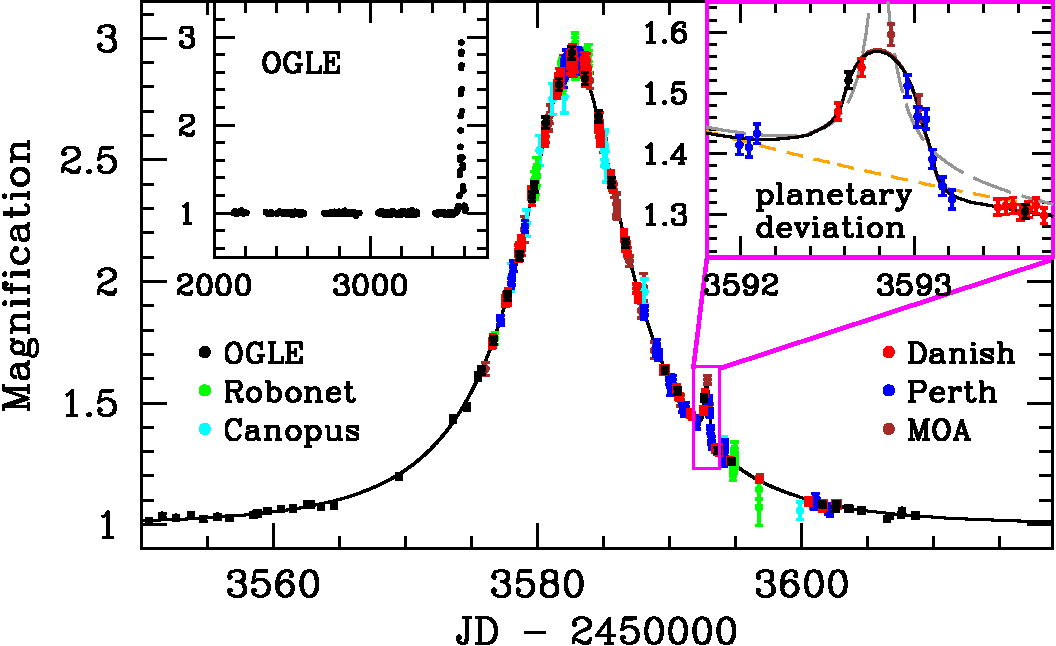
\includegraphics[width=0.5\linewidth]{./figures/introduction/Microlensing_OGLE2005-BLG-390.pdf}
    \caption[Microlensing magnification of OGLE2005-BLG-390.]{Microlensing magnification of OGLE2005-BLG-390 from~\citep{beaulieu_discovery_2006}.
    The presence of the 5.5\,\Mjup{} planet causes the small bump shown in the upper right inset plot.}
    \label{fig:microlensing_example}
\end{figure}

\subsection{Pulsar timing}
\label{subsec:pulsar_timing}
Pulsars are rapidly rotating neutron stars or white dwarfs formed after the death of a giant star, that radiate an intense electromagnetic beam.
The timing variations of the millisecond pulsar\footnote{Rotating at 9\,650 revolutions per minute} {PSR1257+12} led to the first extrasolar planet detection~\citep{wolszczan_planetary_1992}.
There are two models of planet formation around pulsars: either they formed before the supernova explosion and survived, or they formed after, from the remnants of the supernova~\citep{starovoit_existence_2017}.
There is still a rarity of less than 10 pulsars with known orbiting planets.

The rarity of these events is partially associated to the technique which requires very precise instrumentation on high cadence (< milliseconds) to precisely measure the electromagnetic radiation from the pulsar.
For example the first pulsar was detected with the Arecibo radio telescope.
With the primary dish fixed into the mountain, its pointing is limited and achieved by moving the receiver.
It has a limited number of stars that can be observed with a sufficient time coverage to detect planets around pulsars.


%!TEX root = ../../thesis.tex

\section{Detecting atmospheres}
To help characterize an exoplanet, a detection of its atmosphere can provide useful information. After the detection of exoplanets and the measurement of bulk properties, detecting their atmospheres is the next step. The detection of planetary atmosphere is difficult due to the low planet-to-star flux ratio. This requires high precision instrumentation to detect. For example the planet-to-star flux ratio in the optical is $\approx 10^{-4}$ for a hot Jupiter with a 3 day orbit, in which the main component is reflected star light. In the infrared the thermal emission of the planets dominate and the flux ratio rises to $\approx 10^{-3}$. These flux ratios requires observations with signal-to-noise ratios of $10^4$ and $10^3$ in the optical and infrared respectively to achieve a planetary signal at the same level as the noise level. Only just at the capabilities of the current generation of technology, and with very long observation cost.


Several photometric and high-resolution spectroscopic techniques are showing promising results; detailed in the following sections.


\subsection{Occultation and phase variations}
Exoplanet atmospheres are analysis by considering the observed light as containing two components, not only light from the star but also light from the planet, albeit at a much lower flux level.
To help visualize and discuss the components of exoplanet atmospheres \fref{fig:transits_and_occultations} is provided showing a transiting planet in orbit around a star, in which the planet also passes behind the star causing an occultation. The planet is shown at several positions of the orbit indicating the proportion of dayside and night side observed.  Below the star and planet is a diagram showing the changing flux variation over time, following the orbit. 

\begin{figure}
    \centering
    \includegraphics[width=0.6\linewidth]{./figures/introduction/circular_diagram.png}
    \caption{Illustration of the flux contribution from a star and planet in a transiting exoplanet system throughout its orbit. Credit~\citet{winn_transits_2010}}
    \label{fig:transits_and_occultations}
\end{figure}

Throughout the orbit of the planet there is a variation in the planetary flux due to the alternating day/night side of the planet observed.
There are multiple components of the planetary flux, reflection and emission,  that can be analysed with multi-band phase curves \citep[e.g.][]{knutson_characterizing_2009, esteves_optical_2013}. Optical phase curves will mostly show the reflected light from the day side of the planet, allowing modelling the atmospheric albedo (fraction of light reflected by the atmosphere), and can provide details on the atmospheric scattering~\citep{madhusudhan_analytic_2012} and aerosol composition~\citep{oreshenko_optical_2016} through the optical phase function (day/night fraction). Thermal emission of the planet will provide stronger modulation of infrared phase curves and can provide insights into the atmospheres thermal
structure and heat circulation~\citep{ goodman_thermodynamics_2009, koll_temperature_2016 }.


An example of phase variations in infrared spectra obtained with the Hubble Space telescope 
\begin{figure}
    \centering
    \includegraphics[width=0.6\linewidth]{figures/introduction/stevenson_phasecurve2014}
    \caption{Band integrated phase variation of WASP-43b from the HST - \cite{stevenson_thermal_2014}. The primary transit is inset top right.
        The peak of brightness occurs before the secondary transit, indicating heat distribution of the }
    \label{fig:stevensonphasecurve2014}
\end{figure}



The photometric and spectroscopic technique can be understood 
photometric and high-resolution spectroscopicphotometric and high-resolution spectroscopic

Secondary transit and phase variations are an extension of the transit method, requiring higher precision to detect the reflection and thermal emission of the exoplanet. The star with orbiting exoplanet is photometrically monitored over the whole orbit. An example diagram of phase variation is shown in \fref{fig:transits_and_occultations} as the solid black line. Starting with the primary transit at the bottom, in which the planet is blocking the star. The light measured during transit is not only the unblocked light from the star but also the thermal emission from the night side of the planet. Immediately before and after transit there will be the full flux from the star plus the emission from the night side of the planet. As the planet orbits around the star the fraction of the day side of the planet visible will change up to maximum when the full day side of the planet is visible. If the alignment is correct the planet will pass behind the star causing an occultation. At this point the only light received is from the star alone.

The depth of the occultation is a measure of the flux from the day side of the planet which can indicate the atmospheric reflection and thermal emission of the planets atmosphere.
Continuing on in the orbit the phase of combined star + planet again reduces as more of the night side faces Earth.

\fref{fig:stevensonphasecurve2014} shows a real example of the phase folded light curve measured with the HST over several orbits~\citep{stevenson_thermal_2014}.

The primary transit is shown inset with a depth of 2.5\%. The phase variation out of primary transit reaches a maximum of around 0.04\%. The occultation occurs at a phase of 0.5 but it is clearly noticeable that the peak of brightness in the light phase curve slightly leads the occultation. This indicates that the brightest point on the planet is not directly towards the planet. and there is heat redistribution.

thermal profile/phase of hot spot.



\subsection{Transmission spectroscopy}
radius changes with wavelength, extra absorption during transit can give molecular composition.

snellen  et al


Transit and occulations~\citet{winn_transits_2010}

Detection of winds



\citep{hoeijmakers_atomic_2018} detected Iron and titanium in ultra-hot Jupiter with Teff 4000K during transit.high resolution specrosopy






\subsection{High resolution spectroscopy}
Snellen  Brogi, de Kok

Cross correlation mle  \citet{piskorz_evidence_2016}


For non-transiting planets ...



%!TEX root = ../../thesis.tex

\section{Distribution of Exoplanets}

Exoplanetary detections have challenged the theoretical formation models with their variety and distribution of sizes, locations For instance, the discovery of the hot-Jupiter class (large mass planets on close in orbits) challenged the accepted planet formation theories at the time~\citep[.e.g][]{pollack_formation_1996, boss_giant_1997} in which our Solar System was thought to be typical with small rocky planets close to the Sun and large giant planets further away.


The precise characterization of more exoplanets with the detection of exoplanetary atmospheres will allow for the constraints of exoplanetary composition and formation mechanisms to be improved.
For instance, the core accretion model has been able to reproduce the large number of Super-Earths, the correlation be star metallicity and planet frequency~\citep[e.g.][]{santos_spectroscopic_2004, fischer_planetmetallicity_2005}, and the presence of many Hot-Jupiter and Neptune in close-in orbits, with the help of migration mechanisms~\citep[e.g.][]{Triaud_exoplanets_2016}.
Recent models also combine both planetary formation and evolution to describe the observed exoplanets~\citep[e.g.][]{mordasini_characterization_2012} and can reproduce general population properties in a statistically significant way~\citep{mordasini_characterization_2009}.

A proxy for the composition and structure of an exoplanet is the average density, computed from the mass and radius.
A mass-radius diagram is shown in \fref{fig:santerne2018} for Earth-like rocky planets.
The tracks show contours of mass-radius for different theoretical compositions~\citep{brugger_constraints_2017}, while the circles indicate a number of detected small mass exoplanets, with {K2-229\,b} being a Super-Earth with a Mercury-like density~\cite{santerne_earthsized_2018}.
The density can give an approximate composition but for a given mass there are an infinite combinations of metal/silicate/ice and gas that can produce the same radii~\citep[e.g.][]{seager_massradius_2007}.
Low mass planets tend to be rocky and tend to have small or no atmosphere. With rock being in-compressible, to first order, it is relatively insensitive to the incident flux.
The radii of solid exoplanets are sensitive to gas content of the atmosphere as small increase in \ce{H}/\ce{He} can cause a large increase in radius~\citep{adams_ocean_2008}.

When the gas component becomes dominate  planets begin to have radii independent of their mass~\citep[e.g.][]{lopez_understanding_2014}.
The atmospheres of gas giants are also susceptible to stellar irradiation, with close in Hot-Jupiters having inflated atmospheres and larger radii \citep[e.g][]{fortney 2009}. \todo{ Down to here}

\begin{figure}
    \centering
    \includegraphics[width=0.7\linewidth]{figures/introduction/santerne_2018}
    \caption{Mass-Radius diagram for rocky planets with composition contours. Adapted from \citet{santerne_earthsized_2018}}
    \label{fig:santerne2018}
\end{figure}



Models for the mass-radius relation are important as they enable insight into the likely planetary properties when only either mass or radius can or has been measured.
For example \citet{chen_probabilistic_2016} develop a probabilistic model over 9 orders-of-magnitude in mass an 3 orders-of-magnitude in radius.
Their model is shown in \fref{fig:mass_radius_relation}.
It shows ... 4 regions with a split at ... fitted to the data ...

 has been explored out to low-mass stars distribution has been extended out to low-mass stars. 



Brown Dwarfs bridge the gap between low-mass stars and giant planets with masses around \(13-80~\textrm{M}_{jup} \)~\citep{chabrier_theory_2000}, 



Recently, there has been a renewed interest in BD candidates triggered by exoplanetary searches.
While several works found similar properties on the two populations, like a similar density~\citep{hatzes_definition_2015}, others have found intriguing differences.
One of the most recent is the different host metallicity of the Brown Dwarf and giant planet populations~\citep{santos_observational_2017, schlaufman_evidence_2018}, a very strong hint of different formation mechanisms.


Extending the Mass-Radius diagram from low mass planets out to low-mass stars in \fref{fig:mass_radius_relation} reveals interesting situation~\citet{chen_probabilistic_2016}.

There are 4 different regions in which the slow of the M-R diagram is different, potential indicating different formation features with the locations of shle indicating different transition boundaries. \textbf{reread paper} 

\begin{figure}[t]
    \centering
    \includegraphics[width=0.9\linewidth]{./figures/introduction/mass_radius_relation.pdf}  \\
    \caption{Left: Mass-Radius relationship from planets to stars~\citet{chen_probabilistic_2016}.}
    \label{fig:mass_radius_relation}
\end{figure}


\citep{santos_observational_2017} Santos et al 2017 \todo{read and quote}  Observational evidence for two distinct giant planet populations





double peak histogram from an {RV} paper?? Faria 2018?


did they form from the molecular cloud when the star was forming or from the remnants of the disk after the star formed like exoplanets....?






\textbf{brown dwarf dessert explore \citet{ranc_moa2007blg197_2015}}


\subsection{Brown Dwarfs}
\todo{This is mainly from the paper still.}
Brown dwarfs (BDs) are sub-stellar objects unable to achieve hydrogen fusion, with masses around \(13-80~\textrm{M}_{jup} \)~\citep{chabrier_theory_2000}, bridging the gap between low-mass stars and giant planets.
Without sustained fusion, brown-dwarfs cool down over time with an age-dependent cooling rate.
Therefore, there is an inherent degeneracy between the mass, age and luminosity of a given BD~\citep{burrows_nongray_1997}.
This degeneracy may be resolved by the observation of several parameters, for instance when a BD is in a binary system with a main sequence host star, using both the host stars age and the masses derived from the dynamical motion.

A paucity of BD companions exists in short period orbits around Sun-like stars (\(\lesssim5 \)\AU), compared to stellar or planetary companions, termed the \emph{brown dwarf desert}~\citep{halbwachs_exploring_2000, zucker_analysis_2001, sahlmann_search_2011}.
As the number of known BDs orbiting solar type stars is low, the characterization of benchmark BDs in the brown dwarf desert~\citep[e.g.][]{crepp_trends_2016} is beneficial in understanding this sub-stellar population and to help constrain formation and evolution theories~\citep{whitworth_formation_2007}.
The BD desert also provides a greater challenge as it reduces the amount of good BD candidates to study.

BDs in binary systems, unlike free-floating BDs, allow for the determination of their masses, when complemented with radial velocity ({RV}) and astrometry measurements.
The {RV} technique provides the mass lower-limit (\mtwosini{}) of binary and planetary companions, while complementary astrometry measurements can often provide mass upper-limits~\citep[e.g.][]{sahlmann_search_2011}.
Measuring or tightening the constraints of BD masses improves the understanding of mass dependence on BD formation processes.
For instance, there is growing evidence that the larger giant planets and BD companions do not follow the well known metallicity-giant planet correlation seen in main-sequence stars with planets~\citep[e.g.][]{santos_spectroscopic_2004,santos_observational_2017, maldonado_searching_2017}.
Photometry along with stellar evolution models~\citep[e.g.][]{baraffe_evolutionary_2003,allard_btsettl_2013} can also be used to estimate the mass of BD companions~\citep[e.g.][]{moutou_eccentricity_2017} if there is sufficient orbital separation, and a precise determination of the age~\citep{soderblom_ages_2010}.




%
%\begin{figure}[t]
%    \centering
%    \includegraphics[width=0.4\linewidth]{./figures/introduction/Mass_radius_relation-compostion_Brugger_2017.pdf}
%    \caption{Mass-Radius relationship for (super) Earth-like planets with composition contours.
%        Adapted from~\citet{brugger_constraints_2017}}
%    \label{fig:mass_radius_relation_composition}
%\end{figure}



\begin{figure}
    \centering
    \includegraphics[width=0.\linewidth]{./figures/introduction/exoplanetEU_a_mass.pdf}
    \caption{Eoplanet semi-major axis verses mass diagram.
        The symbols indicate the location of the solar system planets, $\mercury$-Mercury, $\venus$-Venus, $\earth$-Earth, $\mars$-Mars, $\jupiter$-Jupiter, $\saturn$-Saturn, $\uranus$-Uranus, $\neptune$-Neptune.
        Data from \href{http://ww.exoplanet.eu}{exoplanet.eu} October 2018}
    \label{fig:pltoverlayadd}
\end{figure}


Explore what these method have found with exoplanet populations.


%!TEX root = ../../thesis.tex

% Motivation of this work
\section{Motivation}


The motivation of this work was to detect the atmosphere of extra solar planets using \nir{} spectra.

This work touches on the RV precision available in the \nir spectra of M-dwarf stars. Following new

%\todo{Pedro: I would only note that you can provide a more detailed description on the importance of determining {RV} information content measurement (at the very end of the chapter)}

%\todo{Nuno: I just think it would be good if you could make the bridge to Brown-Dwarfs and to NIR spectroscopy a bit stronger. Some of the comments and suggestions go in that direction. But since this is an overall suggestion, its not very easy to find the best way through. The general impression one has when reading the introduction is that the thesis is about planets. But then one realizes it is not. But that comes late.}
